\documentclass[aps,twocolumn,secnumarabic,nobalancelastpage,amsmath,amssymb,
nofootinbib,superscriptaddress]{revtex4-1}


\usepackage{graphics}       % standard graphics specifications
\usepackage{graphicx}       % alternative graphics specifications
\usepackage{longtable}      % helps with long table options
\usepackage{url}            % for on-line citations
\usepackage{bm}             % special 'bold-math' package
\usepackage[ngerman]{babel} % deutsche Siblentrennung
\usepackage[utf8]{inputenc} % Umlaute
\usepackage{chemformula}    % für chemische Schreibweise

\def\andname{\hspace*{-0.5em},} % definiert die Trennung zwischen 2 Autoren neu

% Titelseite
\begin{document}
\title{F-Praktikum (Phasendiagramme):\\Differentialthermoanalyse von $\text{Tb}_{0.5}\text{Gd}_{0.5}\text{ScO}_3$
und $\text{Dy}_{0.5}\text{Tb}_{0.5}\text{ScO}_3$\\im Bereich zwischen 300 K und 2300 K}
\author         {Ch. Egerland}
\email[Email: ]{egerlanc@physik.hu-berlin.de}
\author         {M. Pfeifer}
\email[Email: ]{max.pfeifer@physik.hu-berlin.de}
\affiliation    {Humboldt-Universität zu Berlin, Institut für Physik}
\date[Versuchsdatum: ]{05.09.2017}
\date[Versuchsort: ]{Institut für Kristallzüchtung}

%%%%%%%%%%%%%%%%%%%%%%%%%%%%%%%%%%%%%%%%%%%%%%%%%%%%%%%%%%%%%%%%%%%%%%%%%%%%%%%%
\begin{abstract}
Gegenstand dieses Versuches ist die Untersuchung des Temperaturverhaltens der Mischkristalle $\text{Tb}_{0.5}\text{Gd}_{0.5}\text{ScO}_3$ und
$\text{Dy}_{0.5}\text{Tb}_{0.5}\text{ScO}_3$ mittels Differentialthermoanalyse zur näherungsweisen Bestimmung der Schmelzwärmen sowie Schmelztemperaturen.
Die genannten Verbindungen, auch als RE-Skandate ($\text{REScO}_3$, RE=seltene Erde) bezeichnet, werden anschließend in die Systematik der Mischbarkeit von Phasen eingeordnet.
Basierend auf Referenzdaten zu $\text{Gd}\text{ScO}_3$ und $\text{Dy}\text{ScO}_3$ aus [PAPER ALS QUELLE] werden die Schmelzwärmen dieser reinen RE-Skandate mit denen der hier
untersuchten Mischkristalle verglichen.
\end{abstract}


\maketitle


%%%%%%%%%%%%%%%%%%%%%%%%%%%%%%%%%%%%%%%%%%%%%%%%%%%%%%%%%%%%%%%%%%%%%%%%%%%%%%%%

\section{Theorie}
\subsection{Eigenschaften und Struktur von $\text{RESCo}_3$}
\noindent Mischkristalle aus Skandat ($\text{ScO}_3$) und einem seltenen Erdelement (RE), im Folgenden als $\text{REScO}_3$ bzw. RE-Skandate bezeichnet,
finden heutzutage häufig Anwendung bei der Herstellung dünner Perowskit-Filme. Ursache hierfür ist neben der speziellen Kristallstruktur und dem relativ
anspruchslosen Wachstumsprozess v.a., dass nur $\text{REScO}_3$-Mischkristalle Gitterparameter im Bereich zwischen 3.95 \AA$\text{ und}$ 4.02 \AA$\text{ aufweisen.}$
Dabei fällt der Gitterparameter benachbarter $\text{REScO}_3$-Verbindungen mit steigender Ordnungszahl näherungsweise in 0.01 \AA-Schritten. [QUELLE PAPER]

Jedoch sind nicht alle seltenen Erden als Bestandteil von $\text{REScO}_3$-Mischkristallen geeignet ($\text{PmScO}_3$ radioaktiv, $\text{EuScO}_3$ instabil bei Kontakt mit Si).
Außerdem kristallisieren nicht alle RE-Skandate in der Perowskit-Struktur. Nach \cite{perowskHoPr} kann jedoch davon ausgegangen werden, dass solche $\text{REScO}_3$ mit
$\text{RE}=\ch{_{57}Pr}$ bis $\ch{_{67}Ho}$ isomorph sind. Im Gegensatz zur idealerweise kubischen Perowskitstruktur, besitzen diese eine orthorhombische Kristallstruktur.

Um die als Kristallbestandteil ungeeigneten Lanthanoide zu ersetzen, werden Mischkristalle aus jeweils benachbarten RE-Skandaten gezüchtet, so z.B. $\text{Sm}_x\text{Gd}_{1-x}\text{ScO}_3$
für $\text{EuScO}_3$ oder $\text{Nd}_x\text{Sm}_{1-x}\text{ScO}_3$ für $\text{PmScO}_3$ [QUELLE PAPER MESSDATEN]. Werden Mischkristalle gezüchtet, die neben $\text{ScO}_3$ zwei direkt benachbarte
seltene Erdelemente enthalten ($\text{RE1RE2ScO}_3$) ist eine gezieltere Feinabstimmung gewünschter Film-Eigenschaften (z.B. Anpassung Gitterparameter in der Größenordnung von
0.002 \AA$\text{ statt }$ 0.01 \AA$\text{ mit}$ reinen RE-Skandaten) möglich. Dazu werden in diesem Versuch die Verbindungen $\text{Tb}_{0.5}\text{Gd}_{0.5}\text{ScO}_3$
und $\text{Dy}_{0.5}\text{Tb}_{0.5}\text{ScO}_3$ mittels Differentialthermoanalyse untersucht.

\subsection{Differentialthermoanalyse}
\noindent Die Differentialthermoanalyse ist ein thermisches Untersuchungsverfahren zur Materialanalyse. Dabei befindet sich innerhalb eines evakuierten Ofens ein hochtemperaturbeständiger Tiegelhalter
mit zwei symmetrischen Wolfram-Schmelztiegeln: ein Probentiegel mit der zu untersuchenden Substanz und ein leerer (oder mit einer inerten Substanz gefüllten) Referenztiegel. An jedem Probentiegel ist,
wie in Abb. X zu erkennen, jeweils ein Thermoelement aus Wolfram und Rhenium (Schmelzpunkte 3.422 °C und 3.186 °C) angebracht. Wird der Ofen geheizt und dadurch insbesondere eine Temperaturdifferenz an
der Kontaktstelle zwischen W und Re geschaffen, entsteht aufgrund des Seebeck-Effektes eine zur Temperatur proportionale Spannung zwischen den Drahtenden. Findet im Probentiegel nun ein Phasenübergang statt,
der Umwandlungswärme benötigt (1. Art), so steigt die Temperatur dort langsamer an als am Referenztiegel. Durch Reihenschaltung beider
Thermoelemente kann diese Differenzspannung/-temperatur direkt gemessen werden. Nimmt man zusätzlich die absolute Temperatur am Referenztiegel auf, können materialspezifische Eigenschaften der Probensubstanz,
wie Schmeltemperatur und -wärme (Peakfläche) bestimmt werden.

%%%%%%%%%%%%%%%%%%%%%%%%%%%%%%%%%%%%%%%%%%%%%%%%%%%%%%%%%%%%%%%%%%%%%%%%%%%%%%%%

\section{Experiment}
\noindent Untersucht werden 62,85 mg $\text{Dy}_{0.5}\text{Tb}_{0.5}\text{ScO}_3$ und 72,75 mg $\text{Tb}_{0.5}\text{Gd}_{0.5}\text{ScO}_3$, wobei jeweils einmal im Temperaturbereich zwischen 24 °C und 2050 °C
und ein weiteres mal im Bereich zwischen 500 °C und 2050 °C Werte für die Differenzspannung aufgenommen werden. Zur Kalibrierung wurde eine weitere DTA mit $\text{Al}_2\text{O}_3$
durchgeführt, da die Schmelztemperatur von Aluminiumoxid sehr gut bekannt ist. Damit keine Oxidation der Proben stattfindet, finden alle Messungen unter He-Atmosphäre statt.
Die DTA-Messaparatur STA 429 von der Firma NETZSCH wird von einer Steuerungssoftware.. Die Heizrate beträgt 15 K/min.



\begin{figure}[h]
  \centering
  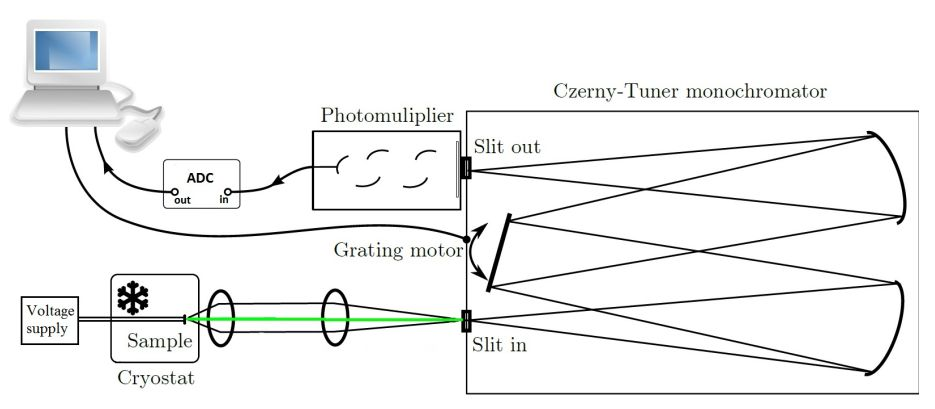
\includegraphics[width=0.48\textwidth]{img/versuchsanleitung.jpg}
  \caption{Versuchsaufbau, aus: \cite{anleitung}}
  \label{fig:versuch}
\end{figure}

\noindent Die durch Rekombination entstandenen Photonen gelangen zunächst durch eine Kollimatorlinse, gefolgt von einer Linse zur
Strahlfokussierung und treffen dann auf ein Czerny-Turner-Monochromator. Durch die Beweglichkeit des Gitters im Monochromator wird


%%%%%%%%%%%%%%%%%%%%%%%%%%%%%%%%%%%%%%%%%%%%%%%%%%%%%%%%%%%%%%%%%%%%%%%%%%%%%%%%

\section{Daten und Analyse}
\subsection{Vorüberlegungen}

\noindent Um eine bessere Einordnung der Ergebnisse zu ermöglichen, wird zunächst mithilfe einer empirischen
Formel die temperaturabhängige Lage des Lumineszenzpeaks (entspricht Größe der Bandlücke) geschätzt.
Hierzu berechnen wir zunächst in welcher Zusammensetzung $\text{Ga}_x\text{In}_{1-x}\text{P}$
an GaAs gitterangepasst ist durch: $a_{GaAs} = x\cdot a_{GaP}+(1-x)\cdot a_{InP}$. Wir finden
$x=0,515$ und mit der empirischen Formel (bei $\text{T}=300\text{ K}$) \cite{vorbereitung}:
\begin{equation}
  E_{g}(x) = 1,351+0,643x+0,786x^2\text{ (eV) }
   \label{eq:Ex}
\end{equation}

\noindent eine geschätzte Bandlückenenergie mit entsprechender Wellenlänge von
\begin{equation}
  E_g \approx 1.89\text{ eV} \Rightarrow  \lambda \approx 656,52\text{ nm}
  \label{eq:evEgap300K}
\end{equation}

\noindent Um nun die Verschiebung von $E_g$ mit der Temperatur zu bestimmen, wurden
die temperaturabhängigen Bandlückenenergien von InP und GaP gewichtet und wir erhalten
die orangene Kurve in Abb. \ref{fig:EgapT} mit einer Differenz zwischen $T=80\text{ K}$
und $T=300\text{ K}$ von:

\begin{equation}
  \Delta E_g \approx 60\text{ meV} \Rightarrow \Delta\lambda \approx 20.0\text{ nm}
\label{eq:evVersch}
\end{equation}

%%%%%%%%%%%%%%%%%%%%%%%%%%%%%%%%%%%%%%%%%%%%%%%%%%%%%%%%%%%%%%%%%%%%%%%%%%%%%%%%
\subsection{Analyse der Spektren}

\noindent Die bei verschiedenen Temperaturen aufgenommenen Spektren sind in Abbildung \ref{fig:spek} dargestellt.
Deutlich zu erkennen ist die Abnahme der Lumineszenzintensität und die Peakverbreiterung bei steigenden Temperaturen.
Oberhalb von ca. $165\text{ K}$ ist ein Verschmieren der linken Peakhälften hin zu kürzeren Wellenlängen zu erkennen.
Deshalb und da bereits ab $T>100$ K ein asymmetrischer Verlauf der Kurven zu erkennen ist, wurden alle Lumineszenzpeaks
einem Doppelgaußfit unterzogen (Mathematica).
Exzitonische Übergänge konnten nicht beobachtet werden. Dies lässt sich leicht
einsehen, wenn man die mittlere kinetische Energie eines Teilchens mit $k_B T\approx 7\text{ meV}$ bei $T=80$ K nähert und
mit der exzitonischen Bindungsenergie (\ref{eq:exitEbind}) vergleicht. Offensichtlich ist die Temperatur
von 80 K zu hoch, um exzitonische Übergänge zu beobachten, da gerade genügend thermische Energie zur Verfügung steht
um die exzitonische Bindungsenergie zu überwinden.

Entscheidend für die Temperaturabhängigkeit der Lumineszenz ist die bei steigenden Temperaturen immer
relevantere Elektron-Phonon-Wechselwirkung. Vernachlässigbar bei geringen Temperaturen sorgen diese Wechselwirkungen
bei großen Temperaturen für die sichtbare Verbreiterung der Peaks (Impulsübertrag von $e^-$ auf Phonon und umgekehrt führt
zu geringfügig niedrigeren/höheren Photonenenergien) \cite{phonons}.

\begin{figure}[t]
  \centering
  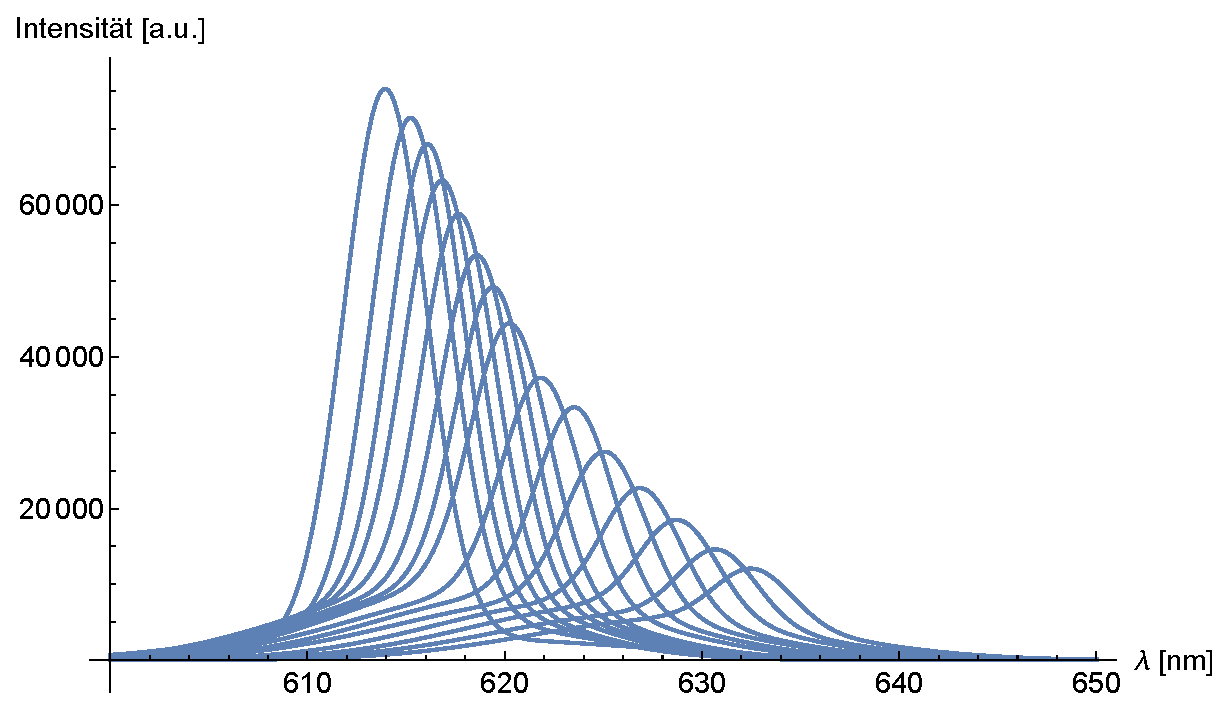
\includegraphics[width=0.48\textwidth]{../Messung/allfitsplot.eps}
  \caption{\label{fig:spek} (1,2-fach) gauß-gefittete Lumineszenzspektren von InGaP zwischen $80\text{ K}$ und $250\text{ K}$ (vlnr)}
\end{figure}

%%%%%%%%%%%%%%%%%%%%%%%%%%%%%%%%%%%%%%%%%%%%%%%%%%%%%%%%%%%%%%%%%%%%%%%%%%%%%%%%
\subsection{Temperaturabhängigkeit der Bandlückenenergie}

\noindent Die Erwärmung des Kristalls führt zu einer Verschiebung der Valenz- und Leitungsbänder und insbesondere
zu einer Verkleinerung der Bandlücke, die gemäß der Varshni-Formel abgeschätzt werden kann:
\begin{equation}
  E_g(T) = E_g(\text{T}=0\text{ K})-\alpha\cdot\frac{T^2}{T+\beta}
   \label{eq:varshni}
\end{equation}

\noindent In den Abbildungen \ref{fig:EgapT} \& \ref{fig:lamT} sind die Temperatur-
abhängigkeiten der Bandlückenenergie und der entsprechenden Wellenlänge dargestellt. Bei steigenden Temperaturen wurde eine deutliche
Rotverschiebung des Intensitätsmaximums gemessen (Verkleinerung der Bandlücke). Die Rotverschiebung konnte auch durch
direkte Beobachtung festgestellt werden. Grund hierfür ist neben der thermischen Ausdehnung des Kristallgitters (Verringerung
der Bindungsenergie der Gitterelektronen/-löcher) die Veränderung des effektiven Kristallpotentials durch bei höheren Temperaturen
zunehmende Elektron-Phonon-Streuung \cite{kittel}.

Führt man eine Extrapolation der experimentellen Daten (Bandlücke/Wellenlänge zwischen 80 K und 255 K) durch und
betrachtet die erwarteten Verschiebungen im Bereich zwischen 80 K und 300 K, lassen sich die Ergebnisse mit (\ref{eq:evVersch})
vergleichen:
\begin{equation}
  \Delta E_{g,exp}\approx 74\text{ meV} \Rightarrow \Delta\lambda_{exp}\approx 23.5\text{ nm}
   \label{eq:expVersch}
\end{equation}

\begin{figure}[t]
  \centering
  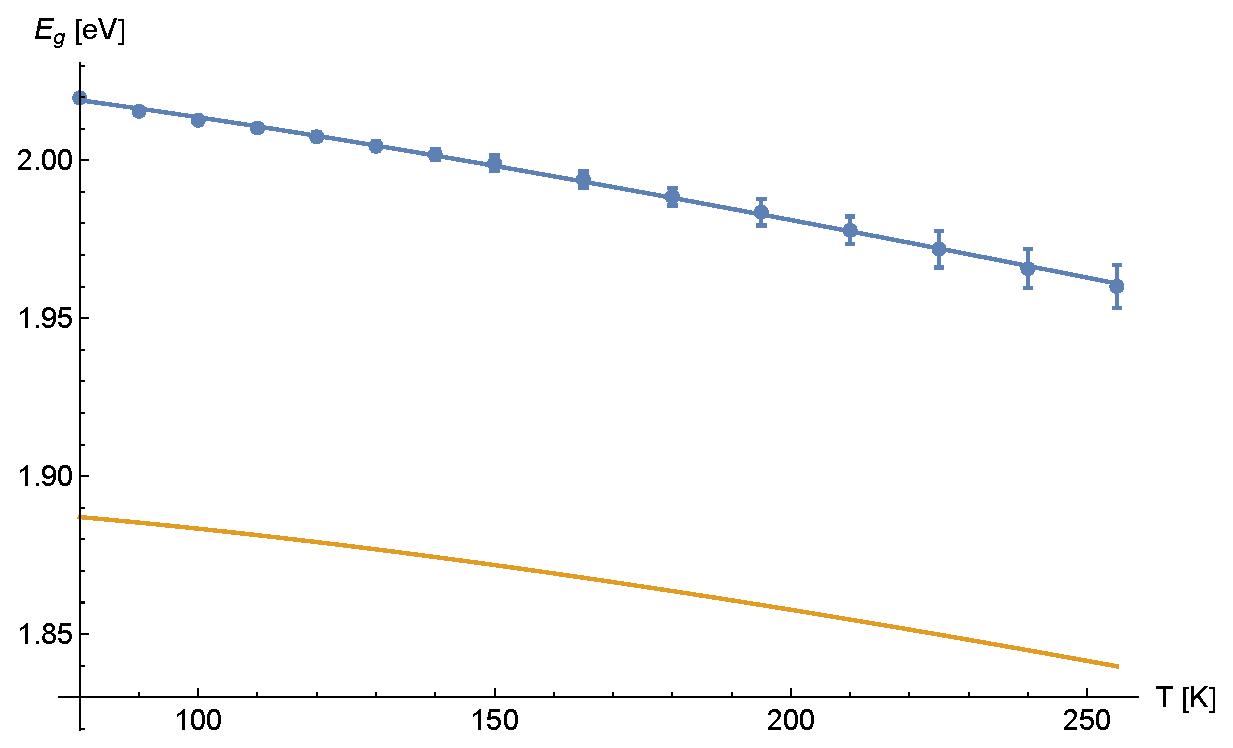
\includegraphics[width=0.48\textwidth]{../Messung/energtemp.eps}
  \caption{\label{fig:EgapT} Bandlückenenergie in Abhängigkeit der Temperatur, Fitparameter
  aus Varshniformel: $E_g^0= 2.03 \text{ eV}$, $\alpha = 4.3*10^{-4}\text{ eV/K}$, $\beta = 140.2 \text{ K}$}
\end{figure}

\noindent Die Größenordnung und Richtung der Wellenlängenverschiebung deckt sich mit der Erwartung aus (\ref{eq:evVersch}).
Die gemessene Änderung der Bandlücke - wie auch die Wellenlängenänderung - ist jedoch etwas größer ausgefallen als die Theorie vorhersagt.
Diese Diskrepanz könnte sowohl von Verunreinigungen des Kristalls als auch von einer abweichenden Materialzusammensetzung als oben angenommen
herrühren. Die konkrete Abweichung der experimentell ermittelten Bandlücke von der Theoretischen gibt Aufschluss über die Mengenverhältnisse von
Ga und In in der Diode. Die Materialzusammensetzung war vermutlich nicht genau gitterangepasst an GaAs, da die erhaltene
Bandlücke experimentell größer ausgefallen ist als theoretisch vorhergesagt (s. Abb. \ref{fig:EgapT}). Neben Verunreinigungen des Materials könnte
die Ursache hierfür gemäß \ref{eq:Ex} ein höherer Gehalt an Ga (GaP) sein (d.h. $x>0.51$).
Extrapoliert man die experimentell ermittelte Bandlücke für $T=300\text{ K}$ mithilfe der Varshni-Formel, lässt sich mit Gl. (\ref{eq:Ex})
ein korrigierter Wert für die Zusammensetzung errechnen. Wir erhalten $x_{korr}\approx 0.55$.

\begin{figure}[h]
  \centering
  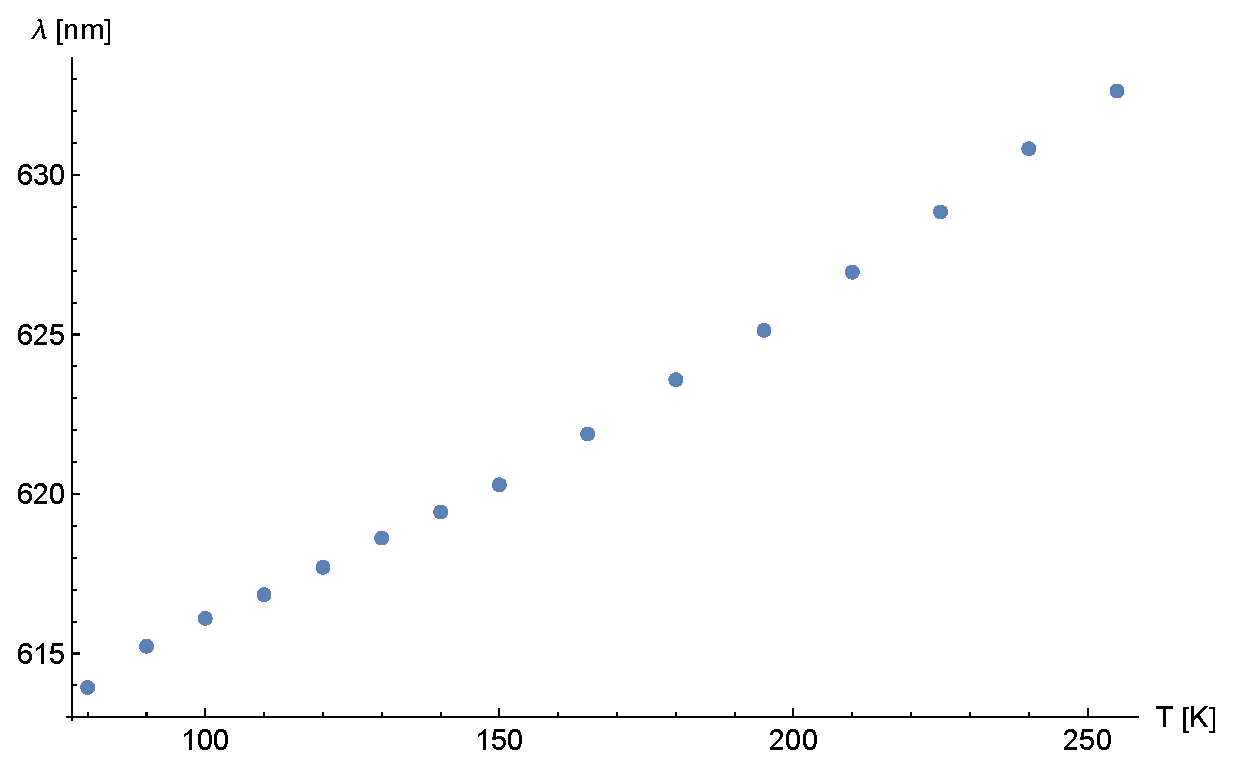
\includegraphics[width=0.48\textwidth]{../Messung/peaktemp.eps}
  \caption{\label{fig:lamT} Temperaturabhängigkeit der Lumineszenz-Wellenlänge von InGaP}
\end{figure}

%%%%%%%%%%%%%%%%%%%%%%%%%%%%%%%%%%%%%%%%%%%%%%%%%%%%%%%%%%%%%%%%%%%%%%%%%%%%%%%%
\subsection{Temperaturabhängigkeit der Intensitäten}

\begin{figure}[b]
  \centering
  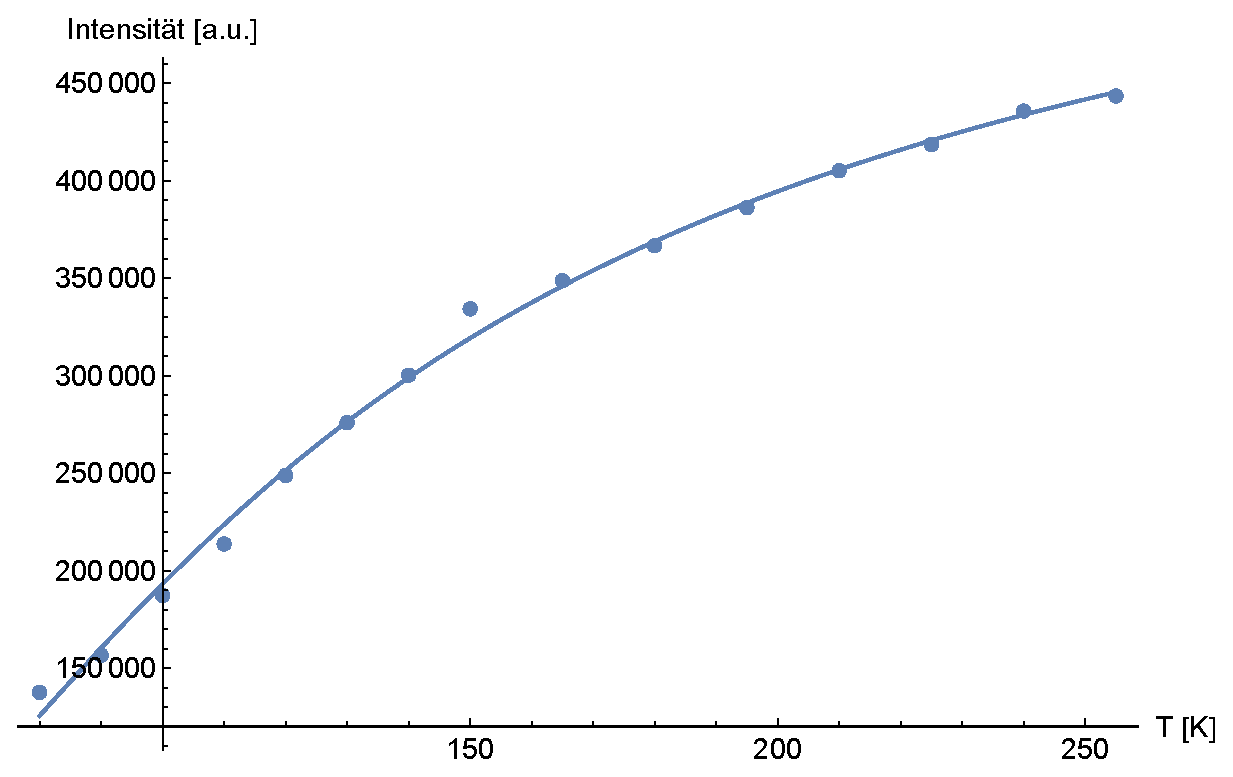
\includegraphics[width=0.48\textwidth]{../Messung/integrintenstempfit.eps}
  \caption{\label{fig:intInt}Integrierte Intensitäten der Lumineszenzpeaks in Abhängigkeit
  der Temperatur,
  Fitparameter aus Arrheniusgleichung: $I_0=450074$, $c=25.2$, $E_A=33.4\text{ meV}$}
\end{figure}

\noindent Die Abnahme der Lumineszenzintensität bei steigenden Temperaturen lässt sich mit der Fermi-Dirac-Verteilung
verstehen: bei steigenden Temperaturen werden zunehmend auch Zustände oberhalb der Fermi-Energie, also Zustände
im Leitungsband bzw. Donatorzustände besetzt, die aufgrund ausreichend thermischer Energie nicht ins Valenzband
rekombinieren und somit für eine Verminderung der Anzahl der abgestrahlten Photonen pro Zeit (und Fläche) sorgen.
Außerdem können aufgrund von Elektron-Phonon-Wechselwirkungen (insb. bei hohen Temperaturen) mehr Ladungsträger durch
Schwingungsrelaxation, also nicht-strahlend, ins Valenzband rekombinieren, was ebenfalls zu einer Reduktion des
Photonenflusses führt.

Die integrierten Intensitäten der Spektrallinien sind in Abb. \ref{fig:intInt} dargestellt. Erkennbar ist
die Abnahme der Peak-Flächen bei steigenden Temperaturen. Mit Hilfe der Arrheniusgleichung lassen sich die integrierten
Peakintensitäten in Abhängigkeit von der Temperatur fitten und somit Rückschlüsse auf die Aktivierungsenergie $E_A$ ziehen.

  \begin{equation}
    I(T) = \frac{I_0}{1+c\cdot\text{exp}\left( -\frac{E_A}{k_B T} \right)}
  \end{equation}

\noindent Diese beschreibt die notwendige Energie eines Ladungsträgers im Donator-/Akzeptorniveau, um ins nächstgelegene Band
(Leitungs-/Valenzband) angeregt zu werden, um dann strahlend, über Phononen oder andere nicht-strahlende Prozesse zu relaxieren.
In Abb. \ref{fig:intInt} ist dieser Fit dargestellt. Wir erhalten eine Aktivierungsenergie von $E_A=33 \text{ meV}$, welche im erwarteten
Referenzbereich von $E_A=(10-50)\text{ meV}$ (für Ga$_{0.52}$In$_{0,48}$P) \cite{eact} liegt.

In Abb. \ref{fig:maxInt} sind die maximalen Intensitäten über die Temperatur aufgetragen. Deutlich ist wieder
der (stärker als lineare) Abfall der Lumineszenz-Intensität bei steigenden Temperaturen. Wie bereits in Abschnitt III.2 erläutert,
sind vor allem Elektron-Phonon-Wechselwirkungen für dieses Verhalten verantwortlich.

\begin{figure}[t]
  \centering
  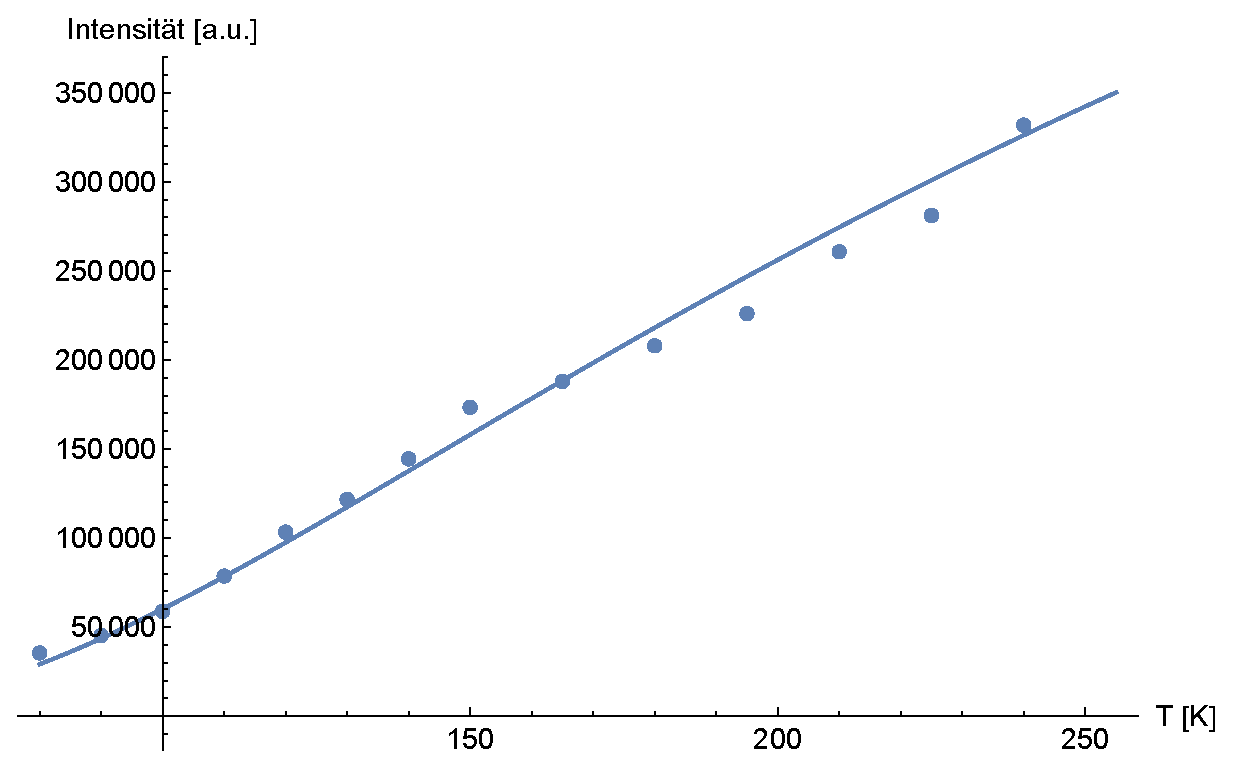
\includegraphics[width=0.48\textwidth]{../Messung/maxintenstempfit.eps}
  \caption{\label{fig:maxInt}Maximale Intensität der Lumineszenzpeaks bei $T=80\text{ K}$ bis $T=250\text{ K}$ (vlnr)}
\end{figure}

%%%%%%%%%%%%%%%%%%%%%%%%%%%%%%%%%%%%%%%%%%%%%%%%%%%%%%%%%%%%%%%%%%%%%%%%%%%%%%%%
\section{Schlussfolgerung}

\noindent Es wurde das Lumineszenzspektrum einer InGaP/GaAs-Photodiode untersucht. Die charakteristische Temperaturabhängigkeit der
Bandlücke, sowie der Peakintensitäten und integrierten Peakintensitäten konnte bestätigt werden. Mittels Vergleich des theoretischen
und experimentellen Temperaturverhaltens der Bandlücke wurde eine Aussage über die Zusammensetzung des Ga$_x$In$_{1-x}$P getroffen
($x>0.51$). Die auf die Lumineszenz bezogene ermittelte Aktivierungsenergie von InGaP liegt im erwarteten Bereich.
Unreinheiten in der Kristallstruktur wurden während der gesamten Betrachtung quantitativ vernachlässigt. Diese würden zur Bildung
von Zwischenniveaus in der Bandlücke führen. Die Absorptionskante würde dadurch, je nach Dotierung, nach oben oder unten verschoben werden, was
zu einer systematischen Abweichung der Bandlücke führen würde.

%%%%%%%%%%%%%%%%%%%%%%%%%%%%%%%%%%%%%%%%%%%%%%%%%%%%%%%%%%%%%%%%%%%%%%%%%%%%%%%%
\bibliography{sample-paper}
\bibliographystyle{prsty}
\begin{thebibliography}{99}
\bibitem{meltpAl2O3}Lide, David R., CRC Handbook of Chemistry and Physics, 83rd ed.; CRC Press: Boca Raton, FL, p 4-39 [2002]
\bibitem{meltpDyScO3}Crnogorac, H. Wilke, Measurement of physical properties of DyScO3 melt, Vol. 44, I 6 [2009]
\bibitem{meltpDyGdScO3}B. Velickov, V. Kahlenberg, R. Bertram, M. Bernhagen, Z. Kristallogr. 222, p 466-473 [2007]
\bibitem{schmelzwAl2O3}Zhang, P.H., Chang, R.Z., Wei, Z. et al. Int J Thermophys 7: 811. https://doi.org/10.1007/BF00503838 [1986]
\bibitem{schmelzwAl2O3_2}Dale L. Perry, Sidney L. Phillips, Inorganic Compounds, CRC Press, p 10 [1995]
\bibitem{perowskHoPr}V.M. Goldschmidt, Naturwissenschaften 14, 477 [1926]
\end{thebibliography}


%%%%%%%%%%%%%%%%%%%%%%%%%%%%%%%%%%%%%%%%%%%%%%%%%%%%%%%%%%%%%%%%%%%%%%%%%%%%%%%%
\clearpage
\appendix
%%%%%%%%%%%%%%%%%%%%%%%%%%%%%%%%%%%%%%%%%%%%%%%%%%%%%%%%%%%%%%%%%%%%%%%%%%%%%%%%


\end{document}
